\documentclass{article}

\usepackage[english]{babel}
\usepackage[utf8]{inputenc}
\usepackage{amsmath,amssymb}
\usepackage{parskip}
\usepackage{graphicx}
\usepackage{listings}
\usepackage{subfig}
\usepackage{float}
\lstset{
    numbers=left, 
    numberstyle= \tiny, 
    keywordstyle= \color{ blue!70},
    commentstyle= \color{red!50!green!50!blue!50}, 
    frame=shadowbox, % 阴影效果
    rulesepcolor= \color{ red!20!green!20!blue!20} ,
    escapeinside=``, % 英文分号中可写入中文
    xleftmargin=2em,xrightmargin=2em, aboveskip=1em,
    framexleftmargin=2em,
    breaklines=true,
    language=R
} 

% Margins
\usepackage[top=2.5cm, left=3cm, right=3cm, bottom=4.0cm]{geometry}
% Colour table cells
\usepackage[table]{xcolor}

% Get larger line spacing in table
\newcommand{\tablespace}{\\[1.25mm]}
\newcommand\Tstrut{\rule{0pt}{2.6ex}}         % = `top' strut
\newcommand\tstrut{\rule{0pt}{2.0ex}}         % = `top' strut
\newcommand\Bstrut{\rule[-0.9ex]{0pt}{0pt}}   % = `bottom' strut

%%%%%%%%%%%%%%%%%
%     Title     %
%%%%%%%%%%%%%%%%%
\title{CSCI946 Assignment}
\author{Yao Xiao \\ SID 2019180015}
\date{\today}

\begin{document}
\maketitle

%%%%%%%%%%%%%%%%%
%   Problem 1   %
%%%%%%%%%%%%%%%%%
\section{Task 1}
\begin{lstlisting}
df <- read.csv("income.csv")

head(df)

# The linear model formula can be written:
#     Income =  7.26299 + 0.99520 * Age + 1.75788 * Education - 0.93433 * Gender
modelA <- lm(Income ~ Age + Education + Gender, data=df)
summary(modelA)

# Call:
# lm(formula = Income ~ Age + Education + Gender, data = df)

# Residuals:
#     Min      1Q  Median      3Q     Max 
# -37.340  -8.101   0.139   7.885  37.271 

# Coefficients:
#             Estimate Std. Error t value Pr(>|t|)    
# (Intercept)  7.26299    1.95575   3.714 0.000212 ***
# Age          0.99520    0.02057  48.373  < 2e-16 ***
# Education    1.75788    0.11581  15.179  < 2e-16 ***
# Gender      -0.93433    0.62388  -1.498 0.134443    
# ---
# Signif. codes:  0 ‘***’ 0.001 ‘**’ 0.01 ‘*’ 0.05 ‘.’ 0.1 ‘ ’ 1

# Residual standard error: 12.07 on 1496 degrees of freedom
# Multiple R-squared:  0.6364,	Adjusted R-squared:  0.6357 
# F-statistic:   873 on 3 and 1496 DF,  p-value: < 2.2e-16
# modelB <- lm(Income ~ Age + Education, data=df)



# The linear model formula can be written:
#     Income = 6.75822 + 0.99603 * Age + 1.75860 * Education
modelB <- lm(Income ~ Age + Education, data=df)
summary(modelB)
# Call:
# lm(formula = Income ~ Age + Education, data = df)

# Residuals:
#     Min      1Q  Median      3Q     Max 
# -36.889  -7.892   0.185   8.200  37.740 

# Coefficients:
#             Estimate Std. Error t value Pr(>|t|)    
# (Intercept)  6.75822    1.92728   3.507 0.000467 ***
# Age          0.99603    0.02057  48.412  < 2e-16 ***
# Education    1.75860    0.11586  15.179  < 2e-16 ***
# ---
# Signif. codes:  0 ‘***’ 0.001 ‘**’ 0.01 ‘*’ 0.05 ‘.’ 0.1 ‘ ’ 1

# Residual standard error: 12.08 on 1497 degrees of freedom
# Multiple R-squared:  0.6359,	Adjusted R-squared:  0.6354 
# F-statistic:  1307 on 2 and 1497 DF,  p-value: < 2.2e-16


# make prediction
prediction <- predict(modelB, item)
prediction
# 1 
# 68.69884 


# compute the confidence interval 
ci <- predict(modelB, item, interval = "confidence")
ci
# fit      lwr      upr
# 1 68.69884 44.98867 92.40902


# compute the prediction interval
pi <- predict(modelB, item, interval = "prediction")
pi
# fit      lwr      upr
# 1 68.69884 44.98867 92.40902
\end{lstlisting}

\section{Task 2}
\begin{lstlisting}
library(pROC)
df <- read.csv("churn.csv")

head(df)

modelA <- lm(Churned ~ Age + Married + Cust_years + Churned_contacts, data = df)
summary(modelA)


modelB <- lm(Churned ~ Age + Married + Churned_contacts, data = df)
summary(modelB)


# The linear model formula can be written:
#     Churned = 0.8226510 - 0.0163168 * Age + 0.0412362 * Churned_contacts
modelC <- lm(Churned ~ Age + Churned_contacts, data = df)
summary(modelC)

# Call:
# lm(formula = Churned ~ Age + Churned_contacts, data = df)

# Residuals:
#      Min       1Q   Median       3Q      Max 
# -0.77637 -0.26017 -0.04805  0.15636  1.13144 

# Coefficients:
#                    Estimate Std. Error t value Pr(>|t|)    
# (Intercept)       0.8226510  0.0133446   61.65   <2e-16 ***
# Age              -0.0163168  0.0002825  -57.77   <2e-16 ***
# Churned_contacts  0.0412362  0.0030280   13.62   <2e-16 ***
# ---
# Signif. codes:  0 ‘***’ 0.001 ‘**’ 0.01 ‘*’ 0.05 ‘.’ 0.1 ‘ ’ 1

# Residual standard error: 0.3441 on 7997 degrees of freedom
# Multiple R-squared:  0.3054,	Adjusted R-squared:  0.3052 
# F-statistic:  1758 on 2 and 7997 DF,  p-value: < 2.2e-16

pre <- predict(modelC, type='response')

# draw ROC
modelCroc <- roc(df$Churned, pre)

plot(modelCroc, print.auc=TRUE, auc.polygon=TRUE, grid=c(0.1, 0.2),
     grid.col=c("blue", "red"), max.auc.polygon=TRUE,
     auc.polygon.col="skyblue", print.thres=TRUE)

# put the predicted probability prob and the actual result y in a data frame
data <- data.frame(prob=pre, obs=df$Churned)

# sort by predicted probability from low to high
data <- data[order(data$prob),]
n <- nrow(data)
tpr <- fpr <- rep(0,n)

# calculate TPR and FPR according to different thresholds
for (i in 1:n) {
  threshold <- data$prob[i]
  tp <- sum(data$prob > threshold & data$obs == 1)
  fp <- sum(data$prob > threshold & data$obs == 0)
  tn <- sum(data$prob < threshold & data$obs == 0)
  fn <- sum(data$prob < threshold & data$obs == 1)
  tpr[i] <- tp/(tp+fn) 
  fpr[i] <- fp/(tn+fp)
}
plot(fpr,tpr,type='l')
abline(a=0,b=1)

\end{lstlisting}

\begin{figure}[H]
    \centering
    \caption{ROC curve}
    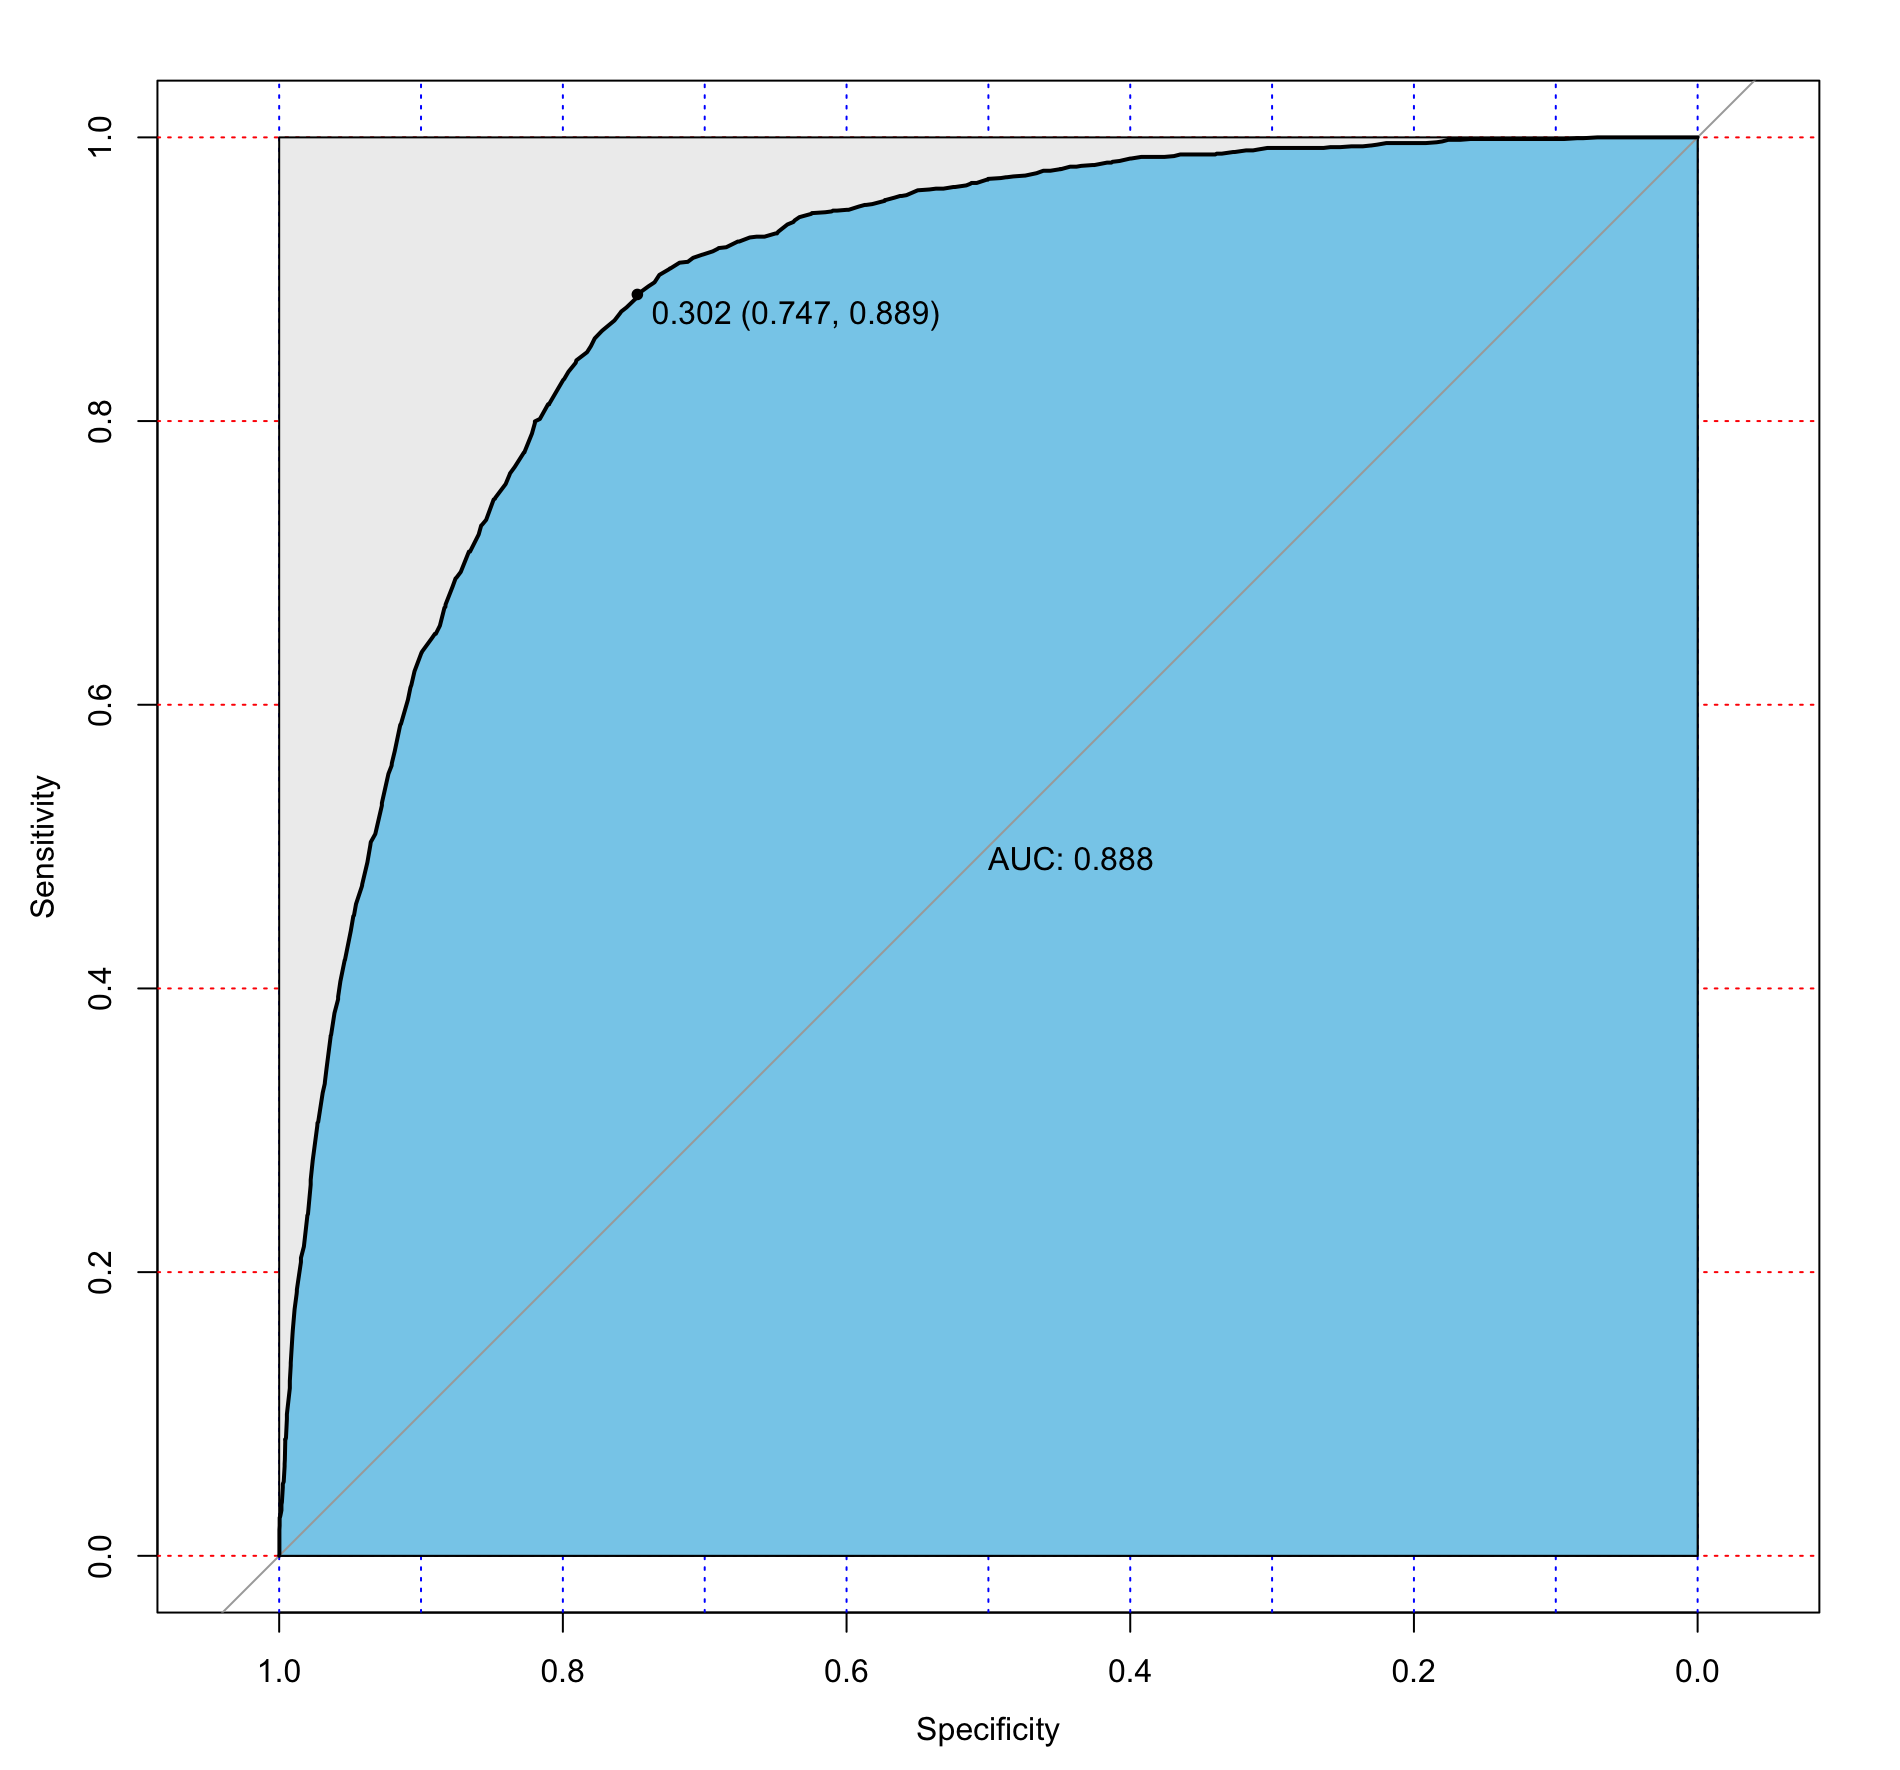
\includegraphics[width=0.85\textwidth]{Fig2}
\end{figure}

\begin{figure}[H]
    \centering
    \caption{FPR and TPR}
    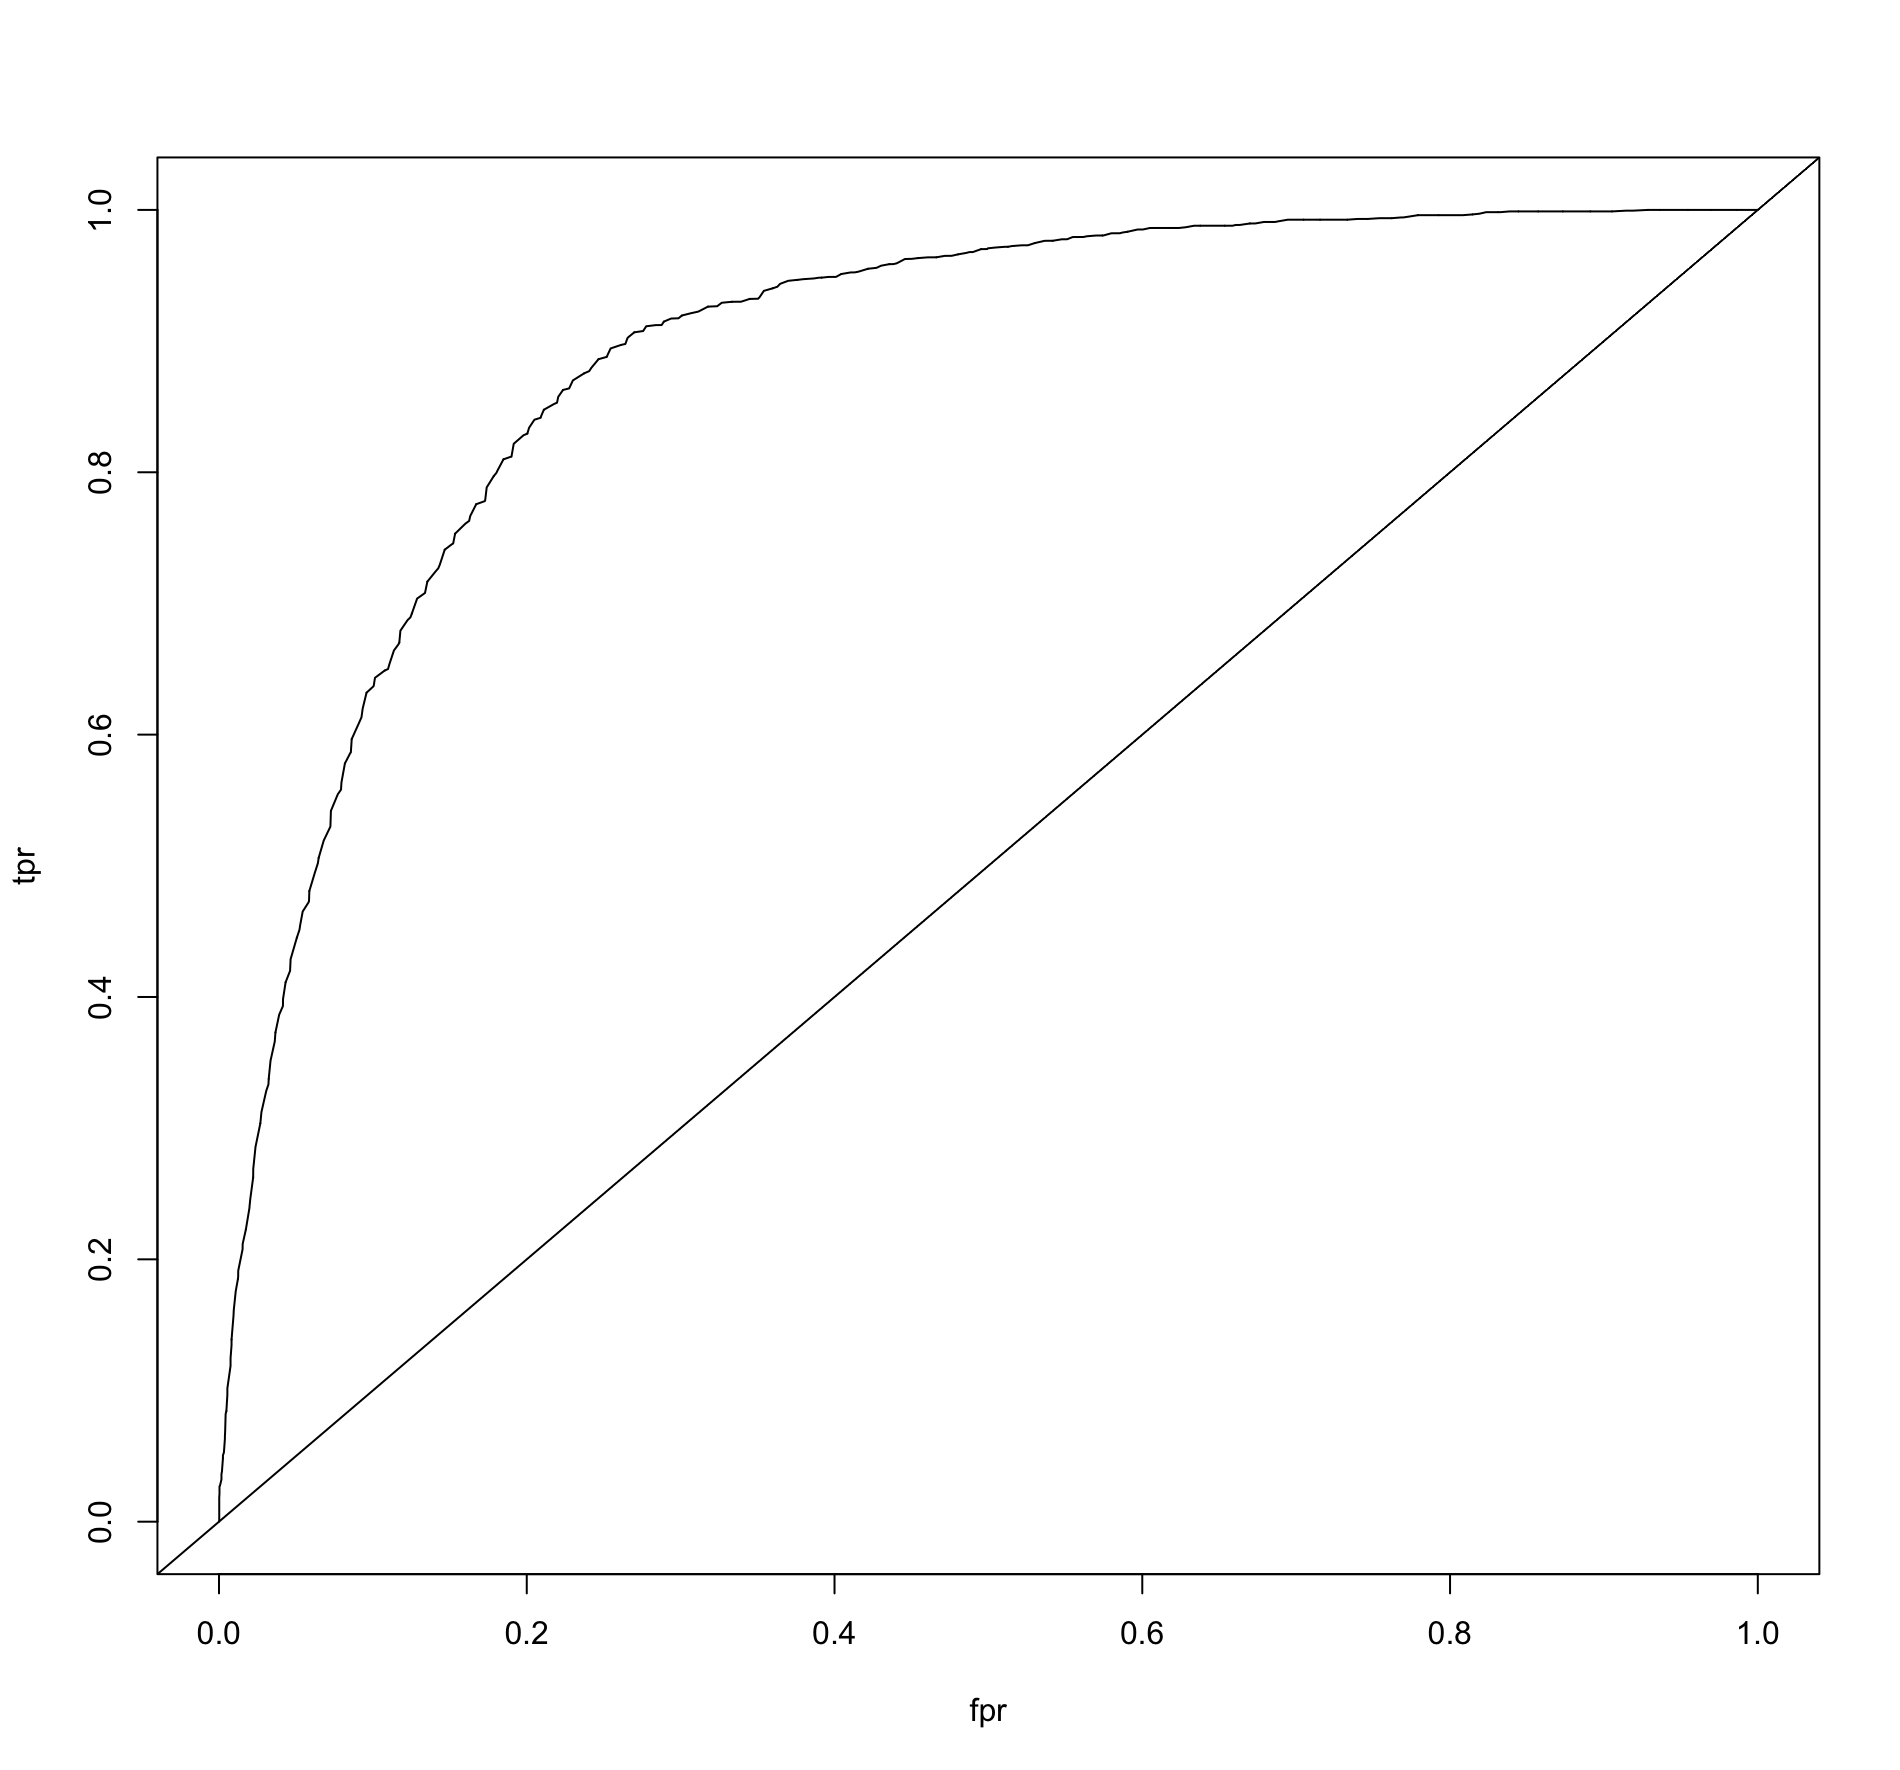
\includegraphics[width=0.85\textwidth]{Fig1}
\end{figure}

\end{document}
